
\input{configuration}

\title{Lecture 10 --- Software Architecture}

\author{Jeff Zarnett\\ \small \texttt{jzarnett@uwaterloo.ca}}
\institute{Department of Electrical and Computer Engineering \\
  University of Waterloo}
\date{\today}


\begin{document}

\begin{frame}
  \titlepage
 \end{frame}
 
 
\begin{frame}
\frametitle{System Design}

\begin{center}
	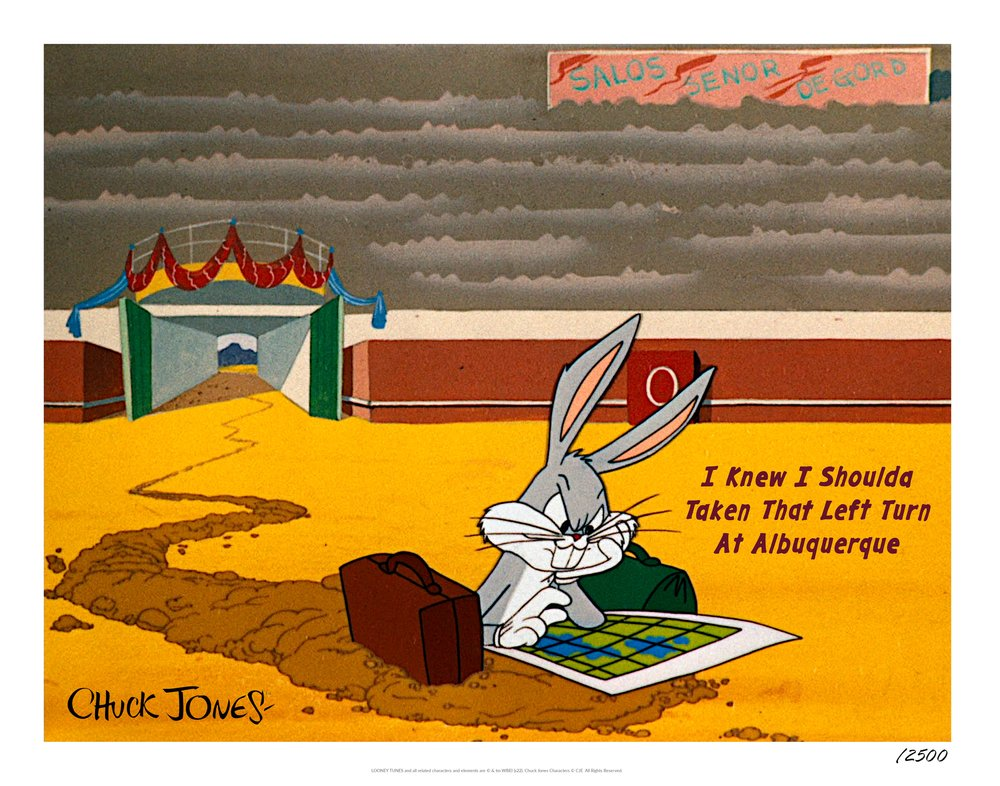
\includegraphics[width=0.7\textwidth]{images/abq.jpg}
\end{center}

Sometimes, the reason that the runtime of some code is what it is results from the design of the larger system in which the data lives.

\end{frame}

\begin{frame}
\frametitle{System Design}
Example: if we need to do lots of network calls to get the data we need, it will be slow compared to locally. What if we can only get items one at a time?

System design interviews are another popular screening method for candidates in industry.

A lot of system design problems are quite open-ended (that's good).

\end{frame}

\begin{frame}
\frametitle{Can I Change That?}
Whether you can change things is very situation-dependent. 

You probably can't convince your boss to rewrite the whole codebase.
\begin{center}
	
\includegraphics[width=0.3\textwidth]{images/jjj.jpg}
\end{center}

It's not even that your argument is necessarily wrong!

Maybe you could change data layout in the database?\\
\quad Or maybe that works for a different use case that's more important.

\end{frame}

\begin{frame}
\frametitle{Another Course?}
Software architecture courses cover this sort of topic in much more depth!\\
\quad Let's think about the implications of architecture on code performance.

High level decisions are rarely made with performance in mind (or a wild guess).

Quick catch-up about monoliths vs microservices...

\end{frame}

\begin{frame}
\frametitle{Architecture Patterns}
Down a level, let's talk about design patterns!

\begin{itemize}
	\item Producer-Consumer?
	\item Blackboard?
	\item Message-passing vs. Shared Memory?
\end{itemize}

Often: boil it down to a real-life analogy. Assembly line?

\end{frame}

\begin{frame}
\frametitle{Implementation}
Zoom in more and we get more decisions to make. Threads? Framework?

Can we choose configuration parameters maybe?

\end{frame}

\begin{frame}
\frametitle{Complexity is the Enemy}

\begin{center}
	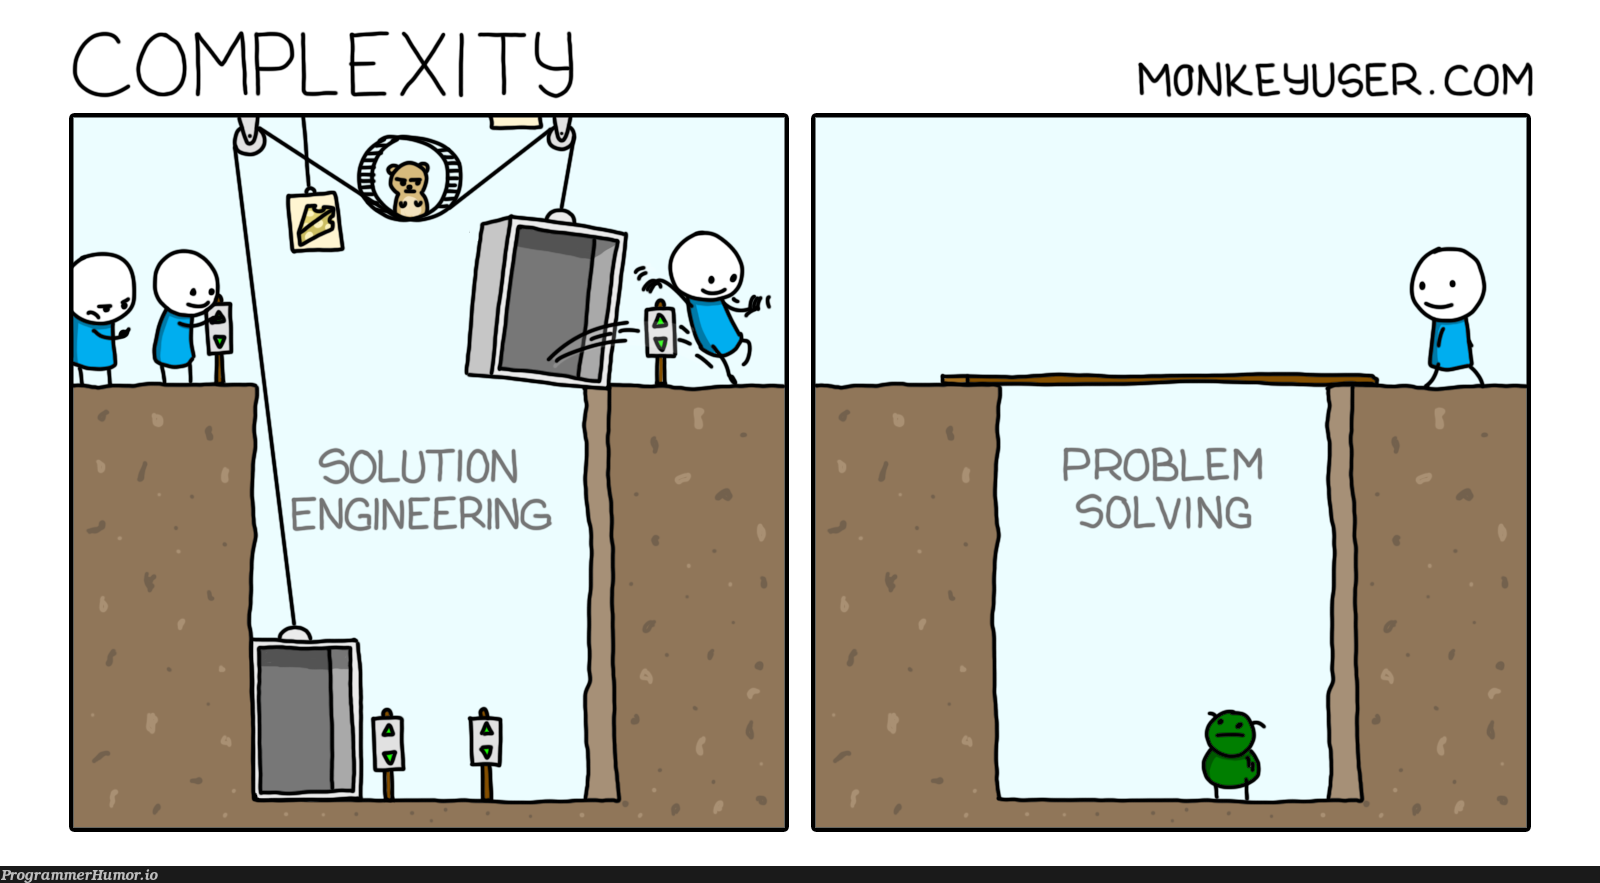
\includegraphics[width=0.8\textwidth]{images/complexity.png}
\end{center}

Complexity is often the result of looking at big companies and thinking their choices are best practices and ``silver bullets''.

\end{frame}

\begin{frame}
\frametitle{Essential and Non-Essential Complexity}
Some complexity is essential: tax software is complex because tax law is complicated and constantly changing!

Other things are our own fault: \texttt{VisitationArrangingOfficer}?!


\url{https://github.com/EnterpriseQualityCoding/FizzBuzzEnterpriseEdition}

\end{frame}
 
 
\begin{frame}
\frametitle{What about Abstraction?}
Abstraction is usually good in software architecture, right?

``We can solve any problem by introducing an extra level of indirection.''\\
\hfill -- David J. Wheeler

Wikipedia even calls it the Fundamental Theorem of Software Engineering.

\end{frame}

\begin{frame}
\frametitle{Abstraction}
\begin{center}
	
\includegraphics[width=0.4\textwidth]{images/thanks.jpg}
\end{center}

Every layer of indirection can easily add additional overhead and result in duplication of work because the right information is not available.

It also slows down the speed of development while you have to just write more stuff to move data around and to keep track of what should be on what level.

\end{frame}

\begin{frame}
\frametitle{They What Now?}
Ancient problem, hopefully died out: \alert{Architecture Astronauts}.

They don't do much directly, but encourage over-engineering and overly-complex solutions. Yikes.

How does that make it slow? More moving data, longer lines of communication!

\end{frame}

\begin{frame}
\frametitle{Pitfalls}

\begin{center}
	
\includegraphics[width=0.8\textwidth]{images/clickbait.jpg}
\end{center}

Four huge architecture mistakes to avoid! Number two will shock you! 

\end{frame}

\begin{frame}
\frametitle{Pitfall 1: Excessive Network Calls}
Reduce the number of network calls to reduce time to completion of requests.

Every call has overhead: establish connection, authenticate, unpack request...

A lot of small requests may be slower than one larger request!

\end{frame}

\begin{frame}
\frametitle{Pitfall 1: Excessive Network Calls}

Minimize the transfer of data, too.

Is this a drawback of microservices? Yes, but rarely a dealbreaker.

Common variant: N+1 query problem.

\end{frame}

\begin{frame}
\frametitle{N+1 Query Problem}

It happens when you want to fetch a list of something, and then for each of those, fetch a list of related entities.

Example: send e-mails to all customers who haven't paid their invoices.

Get unpaid invoices, then find the client for each one, and send them an e-mail.

\end{frame}

\begin{frame}
\frametitle{N+1 Query Problem}
Problem: If there are 500 unpaid invoices, this approach takes 501 queries.

You might say this is easy to avoid:
\begin{center}
	
\includegraphics[width=0.5\textwidth]{images/weaknesses.jpg}
\end{center}

You know about \texttt{JOIN} or \texttt{WHERE... IN} queries!

\end{frame}

\begin{frame}
\frametitle{ORMs Though}

Use an ORM (Object-Relational Mapping)? The framework turns code into some database query statements that you didn't write yourself.

These may unintentionally generate the N+1 variant of your query.\\
\quad It's not on purpose, but you might want to verify.

Solutions: write your own, or enable eager loading.

\end{frame}

\begin{frame}
\frametitle{N+1 Example}

Here's an example from the Sentry Docs:
\begin{center}
  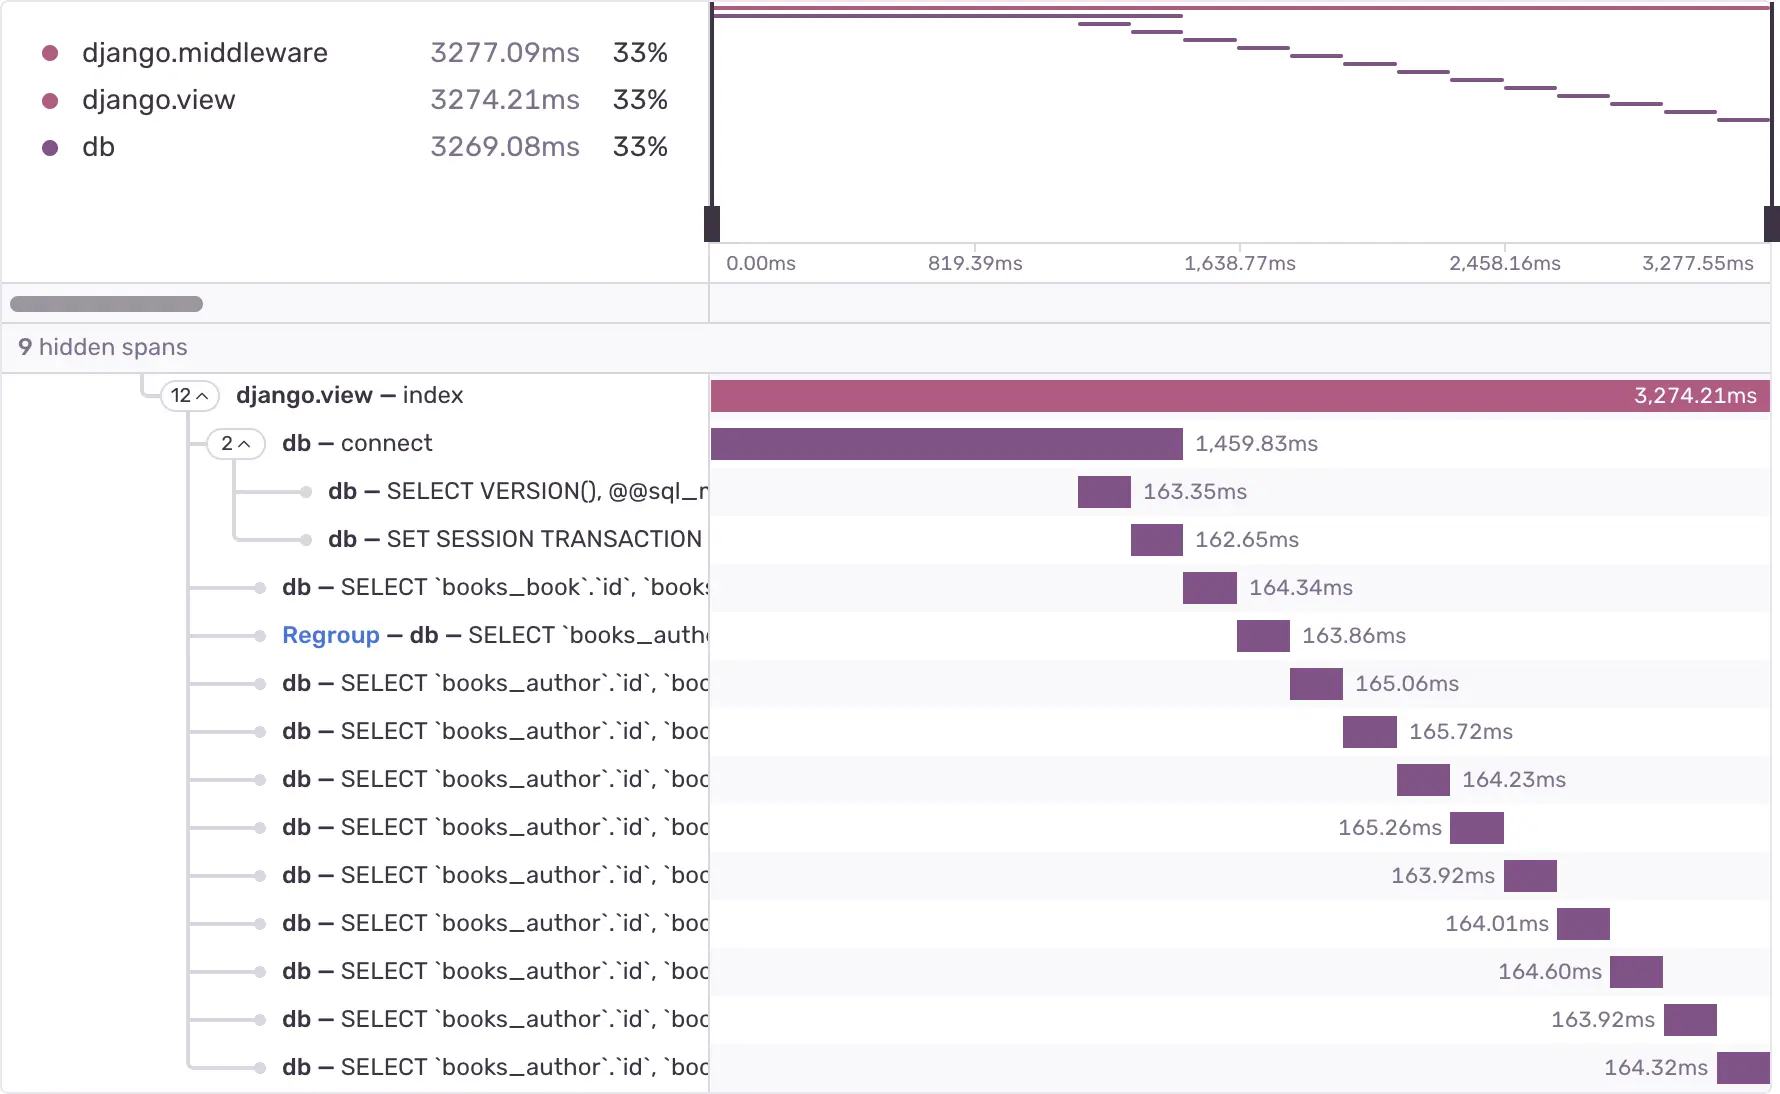
\includegraphics[width=0.7\textwidth]{images/nplusone.png}
\end{center}

\end{frame}

\begin{frame}[fragile]
\frametitle{N+1 Code Example}
The documentation for the Rust crate \texttt{juniper\_eager\_loading} provides a great example of how an N+1 query can result from a GraphQL schema. 


\begin{lstlisting}
schema {
    query: Query
}

type Query {
    allUsers: [User!]!
}

type User {
    id: Int!
    country: Country!
}

type Country {
    id: Int!
    name: String!
}
\end{lstlisting}

\end{frame}

\begin{frame}[fragile]
\frametitle{N+1 Code Example}

And a caller executes the query:
\begin{lstlisting}
query SomeQuery {
    allUsers {
        country {
            name
        }
    }
}
\end{lstlisting}

\end{frame}
\begin{frame}[fragile]
\frametitle{N+1 Code Example}

The naive implementation will run the following queries:
\begin{lstlisting}
select * from users
select * from countries where id = ?
select * from countries where id = ?
select * from countries where id = ?
select * from countries where id = ?
...
\end{lstlisting}

But we actually would prefer...
\begin{lstlisting}
select * from users
select * from countries where id in (?, ?, ?, ?)
\end{lstlisting}

How to solve this?


\end{frame}

\begin{frame}[fragile]
\frametitle{N+1 Code Example}

The core idea is changing how the data structures work to load information if needed but avoid it if it's not.

How do you imagine a user is represented in the system?
\begin{lstlisting}[language=Rust]
struct User {
    id: i32,
    country_id: i32
}
\end{lstlisting}

The only way to get the country name is to load the country...

\end{frame}

\begin{frame}[fragile]
\frametitle{N+1 Code Example}
Alternative that separates the GraphQL models from the Rust structures:

\begin{lstlisting}[language=Rust]
mod models {
    pub struct User {
        id: i32,
        country_id: i32
    }

    pub struct Country {
        id: i32,
        name: String
    }
}

struct User {
    user: models::User,
    country: HasOne<Country>,
}

struct Country {
    country: models::Country
}

enum HasOne<T> {
    Loaded(T),
    NotLoaded,
}
\end{lstlisting}


\end{frame}

\begin{frame}
\frametitle{Finishing N+1 Example}

First, load the users, get a list of country IDs, then query the countries in that set of IDs, and match them up. 

That means replacing the \texttt{User.country} value of \texttt{HasOne::NotLoaded} with \texttt{HasOne::Loaded(matching\_country)}. 

Then we can just return the set of names after the second query.

Much better than the naive approach.

\end{frame}

\begin{frame}
\frametitle{Excessive Network Calls}

Finally, another strategy that reduces the number of network calls is caching.

\begin{center}
	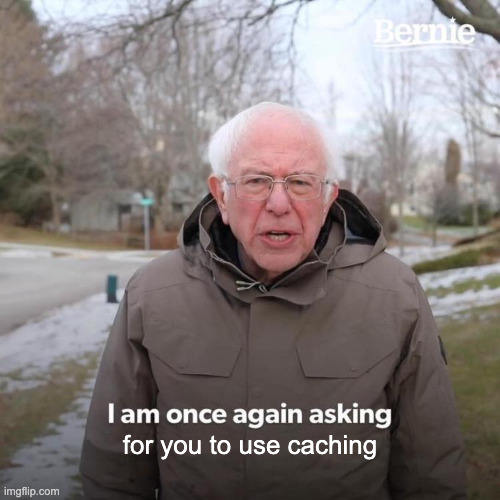
\includegraphics[width=0.5\textwidth]{images/bernie.jpg}
\end{center}

We've discussed it at great length earlier in the course. No need to repeat it.

\end{frame}


\begin{frame}
\frametitle{Pitfall 2: Bottlenecks (Chokepoints)}
Example: authorization service invoked on every API call.

Solution: \texttt{jwt} -- JSON web token that you can validate.\\
\quad It is kind of like a passport.

\begin{center}
	
\includegraphics[width=0.2\textwidth]{images/passport.jpg}
\end{center}

Generalization: can you distribute work?

\end{frame}

\begin{frame}
\frametitle{Pitfall 3: Over-Taking Responsibility}
Searching and filtering in the application is over-taking responsibility.

Why do the job of another component of the system?\\
\quad Let the database do what the database does best.

Another example: doing rendering work in the backend.\\
\quad But remember to validate the frontend input!

\end{frame}

\begin{frame}
\frametitle{Pitfall 3: Over-Taking Responsibility}
That's often caused by organizational or technical constraints.

Examples: gatekeeping or the remote server being another company's code.

Sometimes: trade efficient execution for efficient delivery.

\end{frame}

\begin{frame}
\frametitle{Pitfall 3: Over-Taking Responsibility}

Over-taking responsibility also tends to result in painful change management.

Also: high levels of tech debt if people are afraid of touching a critical system.

No software-architecture decisions can solve organizational problems.

\end{frame}

\begin{frame}
\frametitle{Pitfall 4: Too Much Waiting}

We've already covered asynchronous I/O!

Moving to an asynchronous model is also valuable in reducing \textit{perceived} waits even if the actual execution time is no faster.

Remember \textit{response time}?

\end{frame}

\begin{frame}
\frametitle{Pitfall 4: Too Much Waiting}
Another example: every thread or process waiting to acquire a lock around some shared data. 

Imagine there is one \texttt{Arc<Mutex<Vector>{}>}.

Solution: establish a channel and send the data to one thread.


\end{frame}

\end{document}

